\documentclass[letterpaper,twoside,12pt]{article}
\usepackage[top=1in, bottom=1.25in, left=1in, right=1in]{geometry}
\usepackage{amsmath}
\usepackage{graphicx}
\usepackage{float}

\bibliographystyle{plain}

\title{MAE 766 Computational Fluid Dynamics: Finite Volume Methods for Compressible Euler Equations}
\author{Aditya Kashi}
\begin{document}
\maketitle
\subsection*{Abstract}
In this project, a program to solve two-dimensional compressible Euler equations on triangular unstructured grids has been implemented. Van Leer flux vector splitting is used along with MUSCL reconstruction to try to obtain a second order accurate solution. Van Albada slope-limiter is used to suppress non-physical oscillations at discontinuities. Explicit time integration is done by a 3-stage TVD Runge-Kutta scheme.

\section{Introduction}

Inviscid flow can be described by the compressible Euler equations. The general hyperbolic system is

\begin{equation}
	\frac{\partial \mathbf{u}}{\partial t} + \frac{\partial \mathbf{f}}{\partial x} = 0
\end{equation}
where 
\begin{equation}
	\mathbf{u} = 
	\begin{bmatrix}
		\rho \\ 
		\rho v_1 \\
		\rho v_2 \\
		\rho E
	\end{bmatrix}
\end{equation}
and
\begin{equation}
\mathbf{f}(\mathbf{u}) = 
\begin{bmatrix}
	\rho v_i \\
	\rho v_i v_j + p \delta_{ij} \\
	v_i(\rho E + p)
\end{bmatrix}.
\end{equation}
Here, $\rho$ is the density, $p$ is the pressure, $E$ is the total energy per unit mass and $v_i$ are the velocity components.
The constitutive equation found using the ideal gas law is as follows.
\begin{equation}
	p = \rho (\gamma-1)(E - \frac{|\mathbf{v}|^2}{2})
\end{equation}
$\gamma$ is the adiabatic index $C_p/C_v$.

We let $\Omega$ be the domain of fluid flow and $\Gamma = \partial\Omega$ be the boundary of the domain. Also, let $\mathbf{n}$ denote the outward unit normal vector of the boundary.

Then the weak form of the governing equation is
\begin{equation}
\int_{\Omega} \frac{\partial \mathbf{u}}{\partial t}wd\Omega + \int_{\Gamma} w\mathbf{F_k}\mathbf{n}_k d\Gamma = \int_{\Omega} \mathbf{F}_k \frac{\partial w}{\partial x_k}d\Omega \quad \forall w \in W
\end{equation}
where $w$ is a test function in function space $W$.

\section{Method}

The variational form given above is integrated over each cell for a discontinuous Galerkin formulation.

\begin{equation}
\int_{\Omega_i} \frac{\partial \mathbf{u}}{\partial t}w_h d\Omega + \int_{\Gamma_i} w_h \mathbf{F_k}\mathbf{n}_k d\Gamma = \int_{\Omega_i} \mathbf{F}_k \frac{\partial w_h}{\partial x_k}d\Omega \quad \forall w_h \in W_h \label{weak}
\end{equation}
where the subscript $i$ denotes the ith cell. Now the test function $w_h$ is taken over a single cell.

Given a triangulation of the domain, we solve the discrete version of the variational problem, as described in class \cite{luo}, using a P0 scheme, which is to say that we assume the solutions to be constant over each cell. The problem is semi-discretized in space by a method-of-lines approach using finite volume method, and then integrated in time using a 3-stage TVD (total variation diminishing) Runge-Kutta method.

The boundary integral term in the above equation is evaluated using Van Leer's flux vector splitting scheme, described below. It is evaluated for each face and contributions are `scattered' to the cells sharing that face.

The domain integral is zero in the finite volume case as $w_h$ is constant over each cell.

\subsection{Van Leer Flux Vector Splitting}
Suppose cells $i$ and $j$ share a face, at which we want to calculate the flux (the boundary integral in equation \eqref{weak}). The flux is split and written as
\begin{equation}
f_{ij}(\mathbf{u}_i, \mathbf{u}_j, \mathbf{n}) = f_i^+(\mathbf{u}_i, \mathbf{n}) + f_j^-(\mathbf{u}_j, \mathbf{n})
\end{equation}
We compute the normal Mach numbers for cells $i$ and $j$ as
\[ M_n^i = \frac{v_n^i}{c_i}, \quad M_n^j = \frac{v_n^j}{c_j} \]
Now fluxes are computed depending on these normal Mach numbers, as described in \cite{luo}.

\subsection{MUSCL Reconstruction}
In case of the reconstructed (2nd order) finite volume (or rDG P0-P1) scheme, the gradient has been reconstructed in each cell using a weighted least-squares reconstruction from values of unknowns at face-neighboring cells. For cells having a boundary face, ghost cell centroids and boundary data were calculated and used to reconstruct the gradient in those cells.

To suppress non-physical oscillations at discontinuities in the solution, the van Albada slope limiter was used.

\subsection{Code}
The implementation was coded from scratch in C++ (version 11). A templated matrix-manipulation class was written first, to make array handling easier. A mesh class was implemented to read the mesh file and calculate mesh data structures such as points surrounding points, elements surrounding elements, face data structure relating to cells, Jacobians of the cells etc. These were used in implementing the basic finite volume and MUSCL-reconstructed finite volume schemes described earlier. ParaView (Kitware, inc.) was used for visualization.

\section{Results}

First, subsonic flow over a cylinder was simulated and a grid-refinement study was done,shown in figures \ref{order} and \ref{order-recons}. Mach number has been plotted for this case (figure \ref{cyl-mach}).

\begin{figure}[!H]
	\centering
	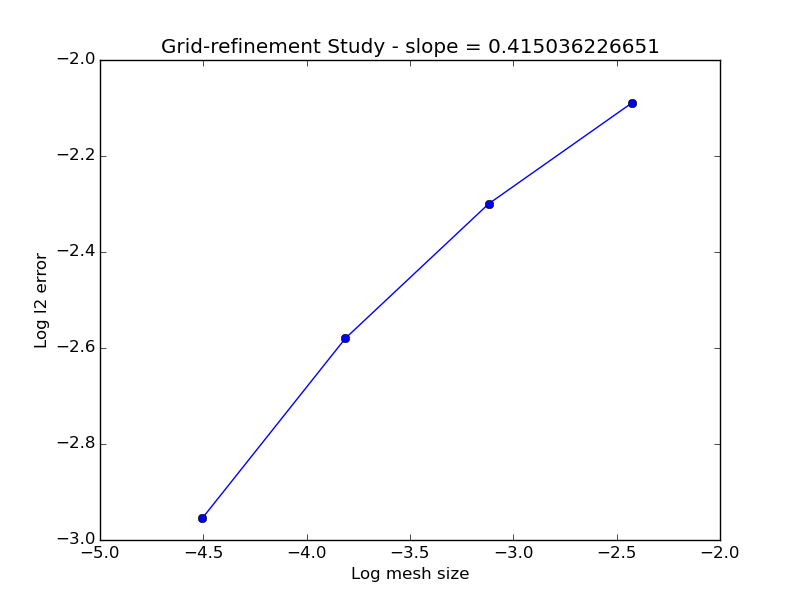
\includegraphics[scale=.5]{convergence-reconstructedFV}
	\caption{Grid-refinement plot for reconstructed finite volume scheme}
	\label{order-recons}
\end{figure}

\begin{figure}[!H]
	\centering
	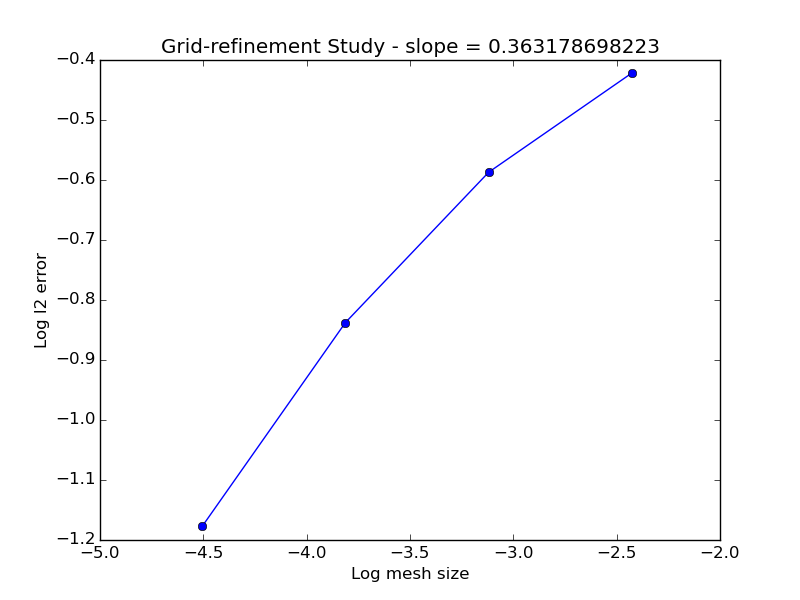
\includegraphics[scale=.5]{convergence-FV}
	\caption{Grid-refinement plot for basic finite volume scheme}
	\label{order}
\end{figure}

\begin{figure}[!H]
\centering
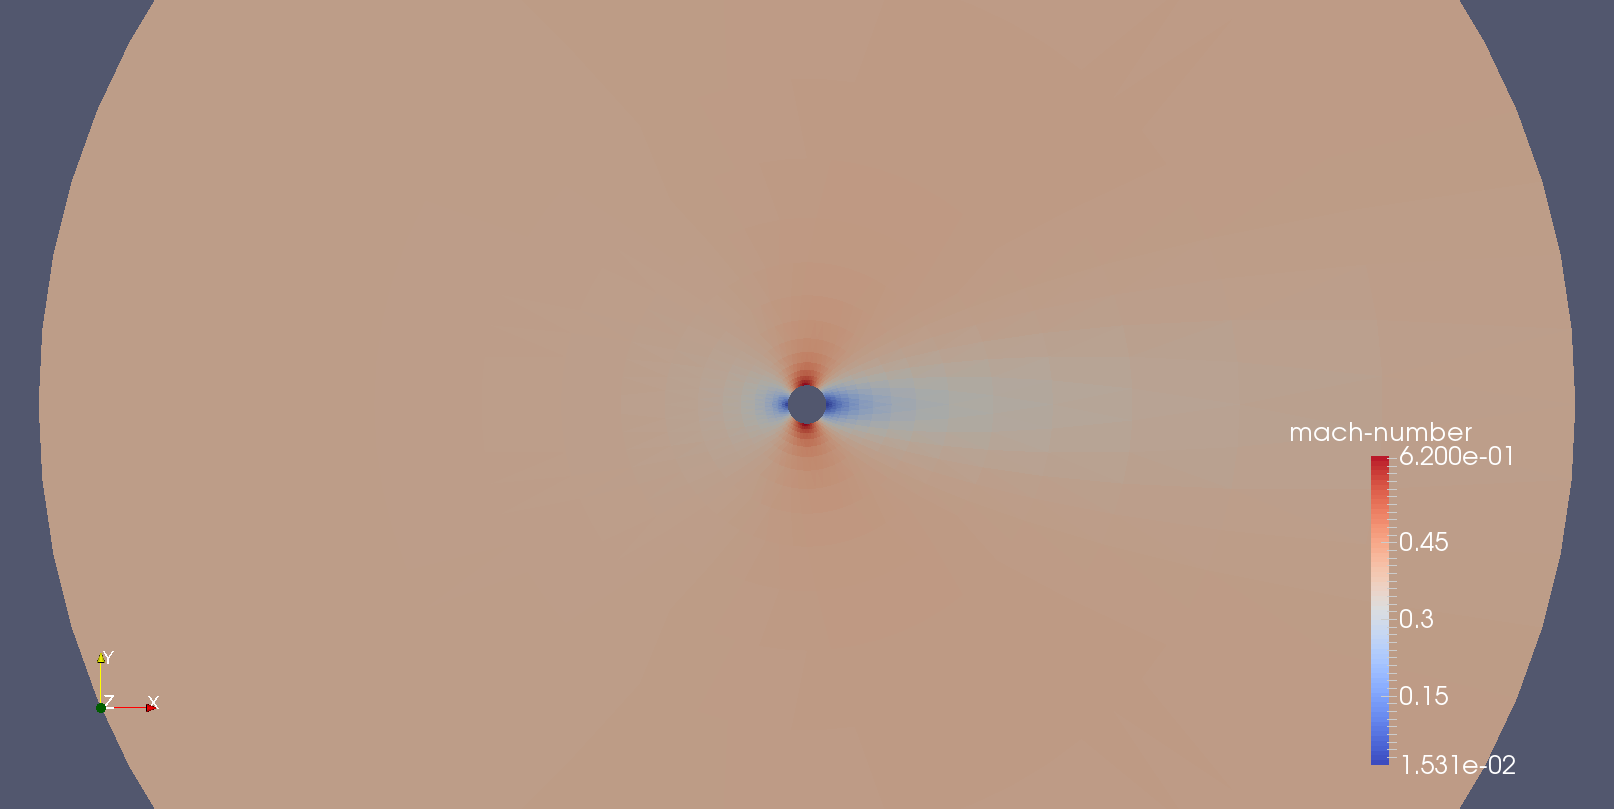
\includegraphics[scale=.25]{cyl-fine-2}
\caption{Mach number plot for subsonic flow over a cylinder}
\label{cyl-mach}
\end{figure}

Next, Mach number and pressure have been plotted for supersonic (M=1.1) flow through a bump-channel (figures \ref{bump-mach} and \ref{bump-pressure}).

\begin{figure}[!H]
\centering
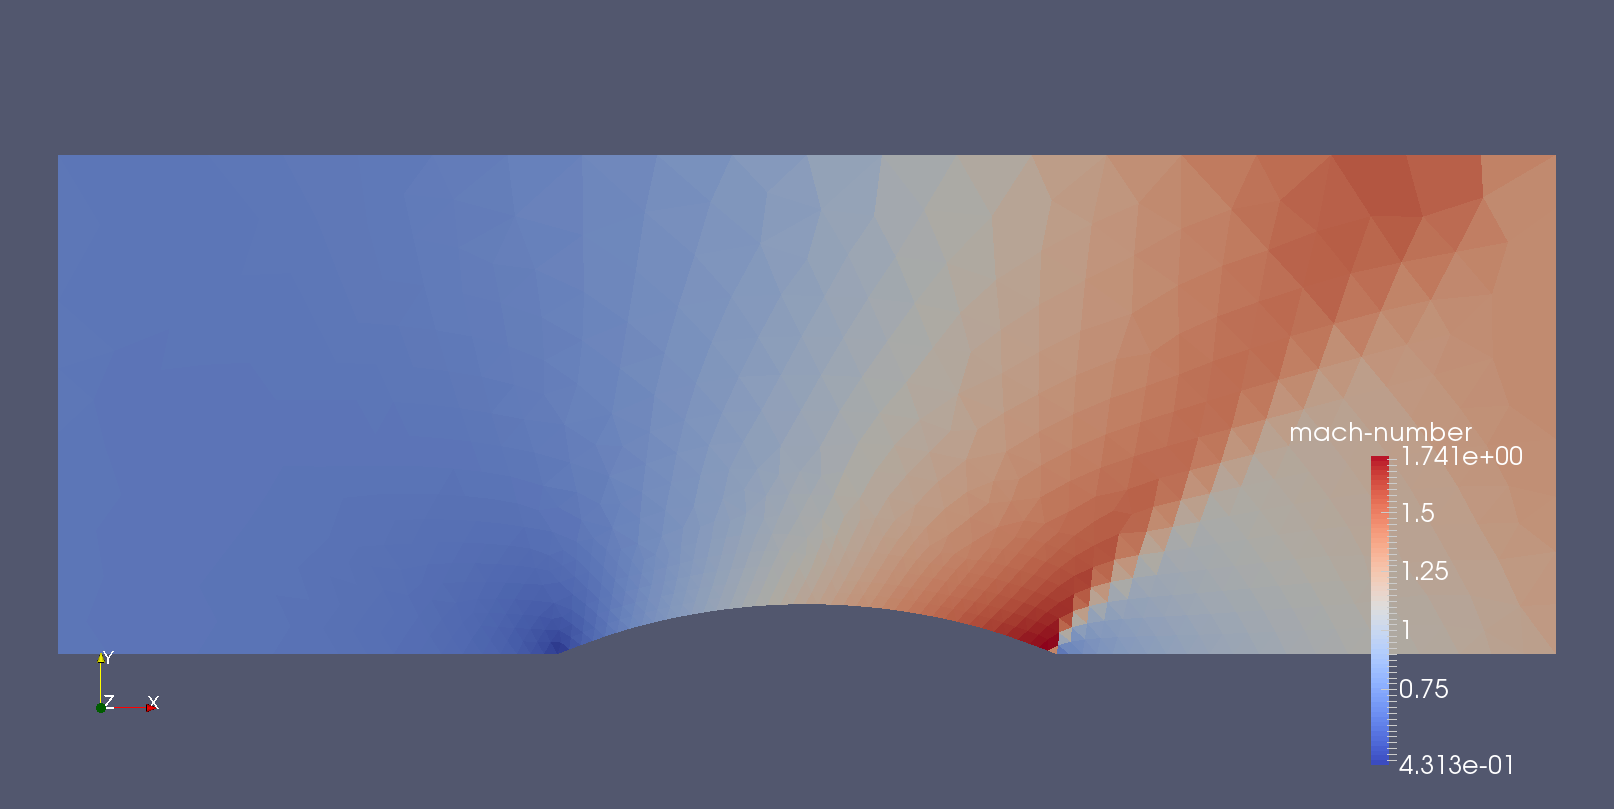
\includegraphics[scale=.25]{bump-2-mach}
\caption{Mach number plot for supersonic flow through bump channel}
\label{bump-mach}
\end{figure}

\begin{figure}[!H]
\centering
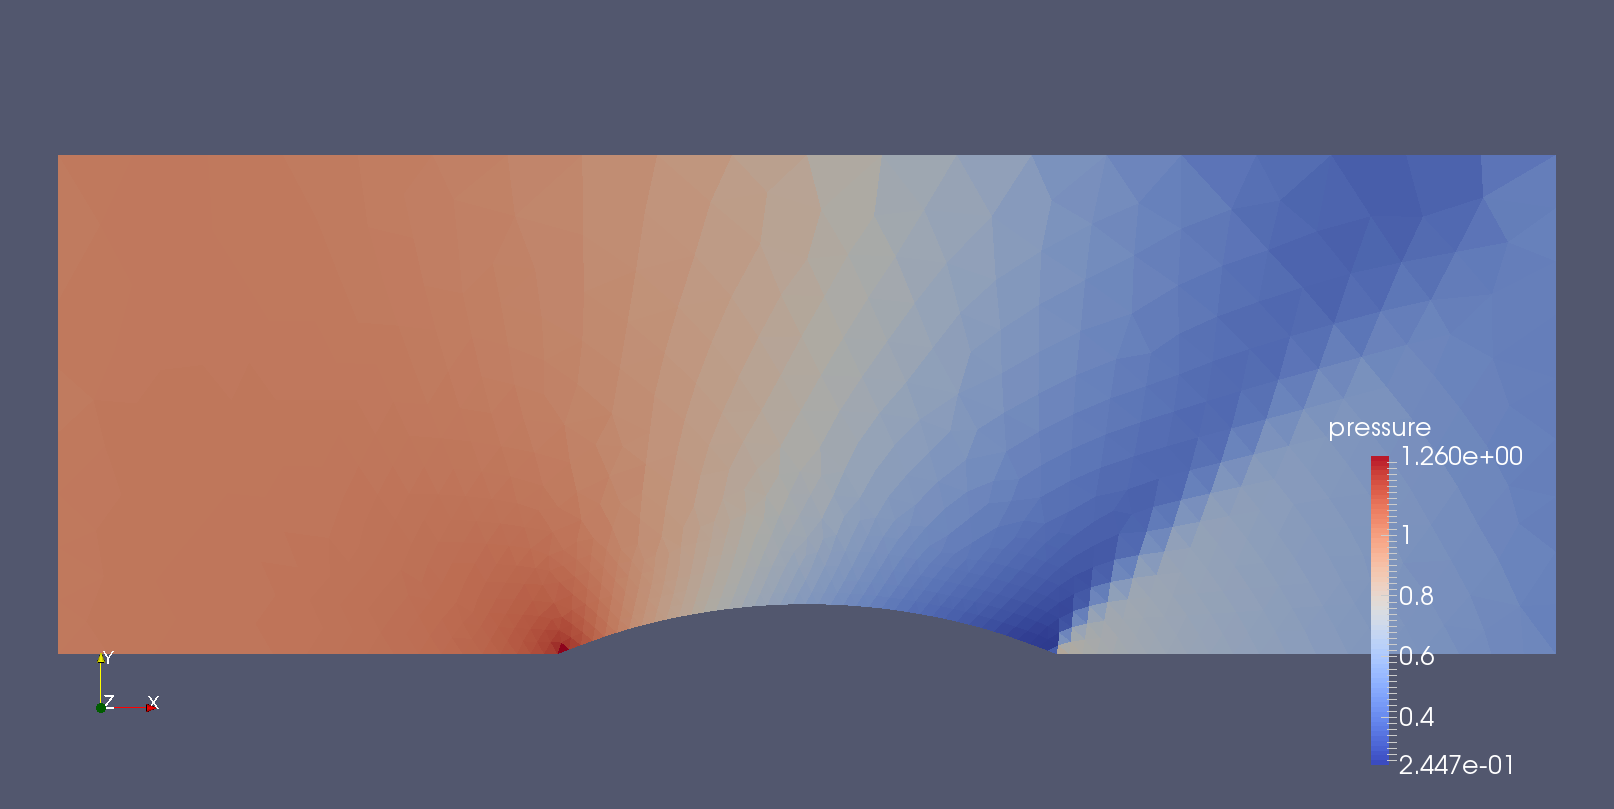
\includegraphics[scale=.25]{bump-2-pressure}
\caption{Pressure plot for supersonic flow through bump channel}
\label{bump-pressure}
\end{figure}

Finally, Mach number and pressure plots are shown for transonic (M=0.85) flow over a NACA0012 airfoil (figures \ref{naca-mach} and \ref{naca-pressure}).

All of the 2D contour plots correspond to the reconstructed finite volume simulations.

\begin{figure}[!H]
	\centering
	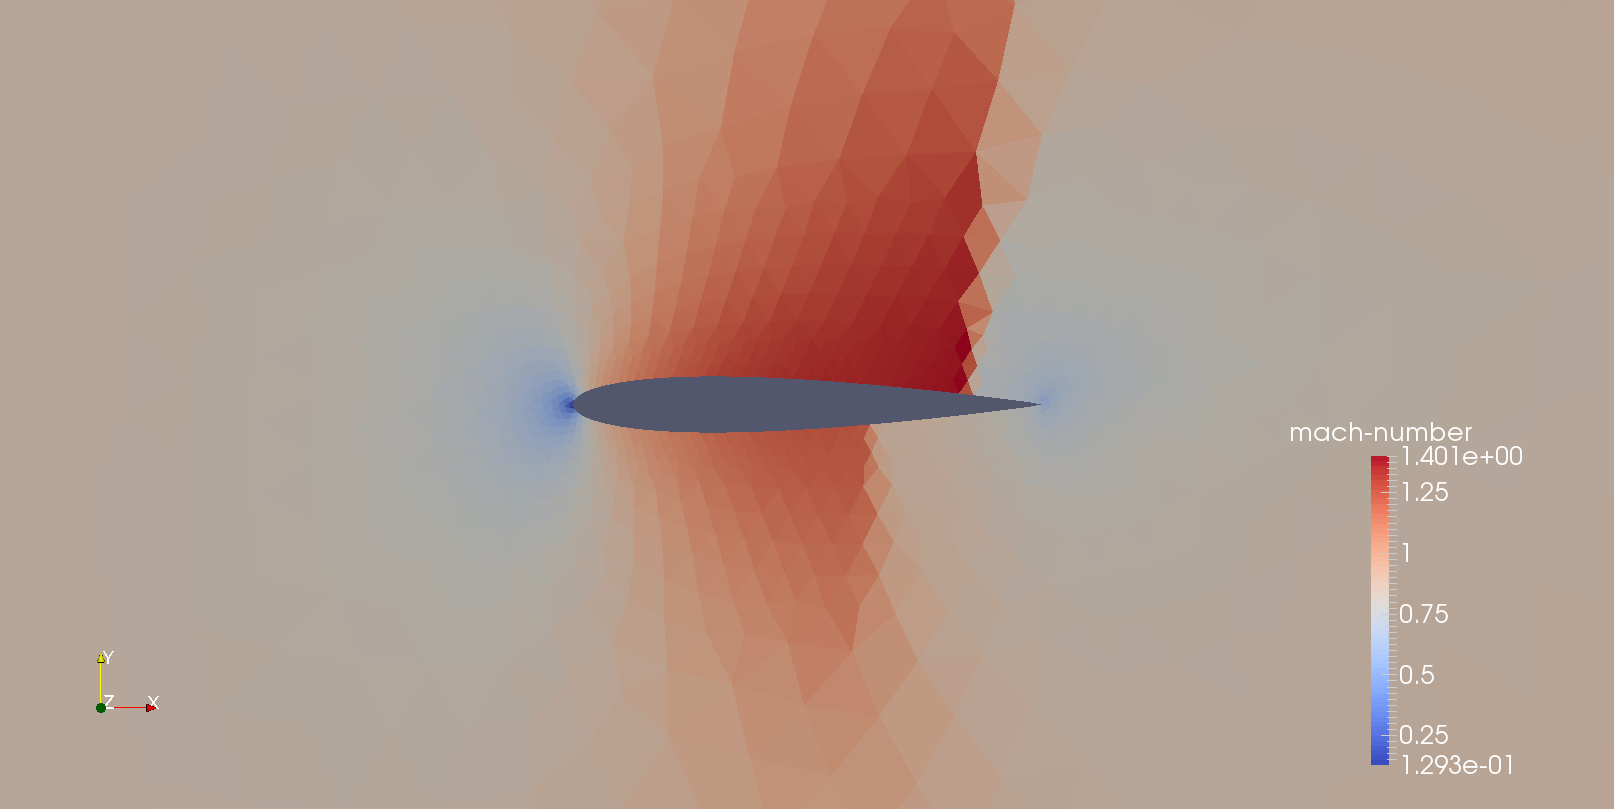
\includegraphics[scale=.25]{naca12-2-mach}
	\caption{Mach number plot for transonic flow over NACA0012 airfoil}
	\label{naca-mach}
\end{figure}

\begin{figure}[!H]
	\centering
	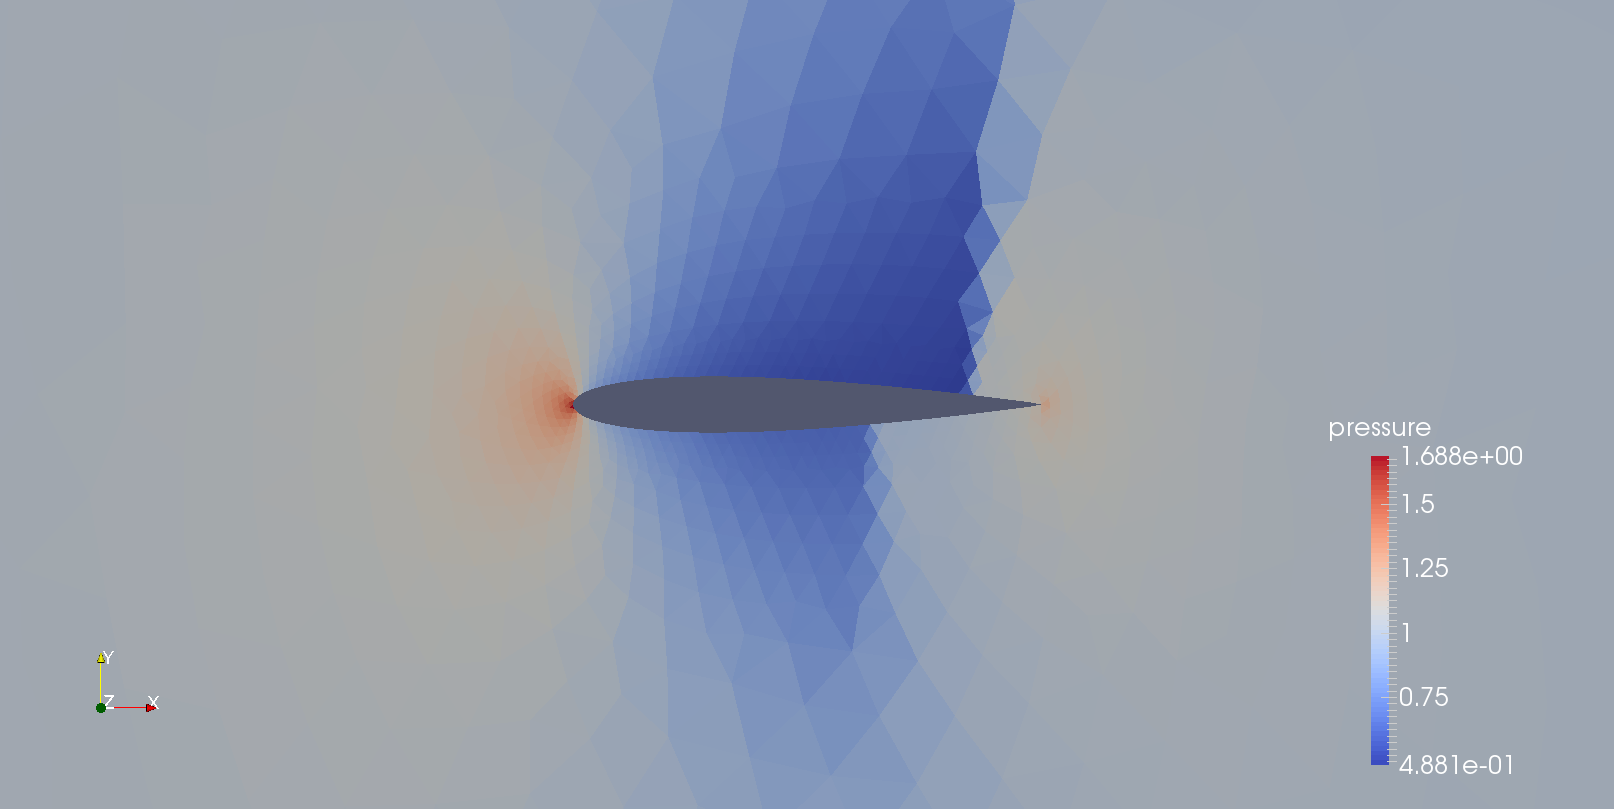
\includegraphics[scale=.25]{naca12-2-pressure}
	\caption{Pressure plot for transonic flow over NACA0012 airfoil}
	\label{naca-pressure}
\end{figure}

As can be seen, the orders of accuracy (0.36 for DG P0 and 0.42 for rDG P0-P1) are quite low. The author has not yet identified the sources of inaccuracy, which will be accomplished soon.

\bibliography{references}

\section*{Acknowledgements}
I am very thankful to my advisor and course-instructor Professor Hong Luo for always welcoming my doubts and clearing then. I am also thankful to my lab-mates Chad Rollins, Xiaodong Liu and Aditya Pandare for discussing some implementation issues.

\end{document}